\chapter{Metodoloxía e planificación}
\label{chap:metodoloxia}

\hfill\emph{O que queira peixes que molle o cu} \cite{peixe}

\lettrine{N}{este} capítulo descríbese cómo se traballou así como os recursos involucrados e a planificación do traballo.

\section{Método de traballo}

\begin{figure}
  \centering
  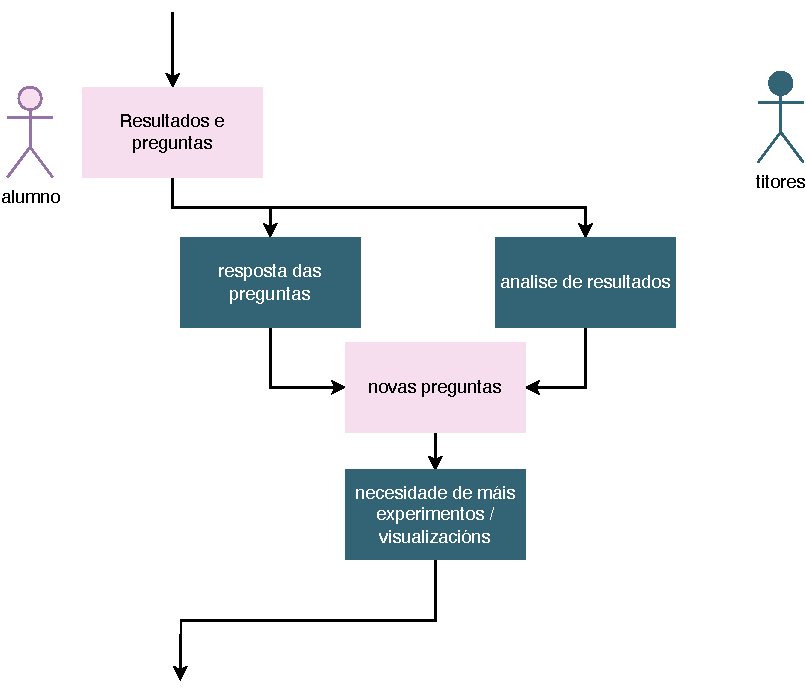
\includegraphics[width=0.6\textwidth]{imaxes/metodoloxia.drawio.pdf}
	\caption{Esquema do contido das reunións semanais entre o alumno e os titores.}
	\label{fig:metodoloxia}
\end{figure}

Os primeiros esforzos adicaronse á compresión do material. Unha vez a compresión foi sufiente para empezar as iteracións semanais, estas consistían en sucesións de reunión (ver \ref{fig:metodoloxia}) e traballo individual. O traballo individual do alumno ó longo das semanas comprendía:
\begin{itemize}
				\item \textbf{Programación:} de experimentos (isto é: adestramento de \acrshort{rna}) e de visualizacións para poder analizar distintos aspectos das Redes adestradas.
				\item \textbf{Análise de resultados:} para interpretar as visualizacións e formular afirmacións ou preguntas dependendo do entendemento. En ambos casos era moi útil porque se formulaba unha afirmación, ó presentarlla ós titores ou ben comprendía porque tiña razón ou porque non a tiña; e se formulaba unha pregunta aprendía da súa resposta.
				\item \textbf{Lectura bibliográfica:} de temas que non plantexáronse ó principio pero foron importantes para respostar ás preguntas que xurdían e en xeral comprender profundamente o tema a tratar, segundo íase presentando de forma distinta ó longo das semanas.
\end{itemize}


\section{Recursos}
\subsection{Humanos}
Este traballo foi supervisado por tres tutores \footnote{Un dos cales mudou de universidade durante o traballo e por tanto non figura na portada.} que tiveron o rol directivo en canto ás ideas, respostaron a pregunta `Qué se fai?' e en canto o método, `Cómo se fai?'. O alumno tivo de entrada un natural papel subordinado é dicir, leu e programou o que se lle mandou. Co paso das semanas, o coñecemento e intuición que desenvolveu o alumno sobre o tema permitiulle do mesmo modo propoñer ideas e métodos, dotando ós tutores dun rol máis alto nivel.

A primeira achega dos tutores foi o punteiro á bibliografía e código necesarios para a compresión do tema. Devandita tarefa mantivo ocupado ó alumno en soidade os primeiros meses e cando este acadou un nivel de compresión sufiente comenzaron as reunións semanais. Estas seguían o esquema da Figura \ref{fig:metodoloxia}


\subsection{De \emph{Software}}

A continuación listanse os recursos \emph{Software} empregados no traballo con importancia descendente. Nótese que todo o \emph{Software} é código aberto e nalgúns casos código libre.


\begin{itemize}
				\item \textbf{Python:} \footnote{Python Software Foundation License Version 2 (PSF-2.0)\label{fn:psf}} a linguaxe por defecto para escribir os programas do traballo. Funcionalmente é conector das librerías mencionadas xa que se ben por si só Python non é tan útil para a práctica de \acrshort{aprpro}, funciona como un fabuloso pegamento.
				\item \textbf{PyTorch:} \footnote{BSD 3-Clause License\label{fn:bsd3}} a libraría por defecto de \acrshort{aprpro} hoxe en día que permitiunos facer modificacións, inspeccións e adestramentos sobre a \acrshort{rna}, o cal corresponde co \emph{grosso} do traballo.
				\item \textbf{einops:} \footnote{MIT License\label{fn:mit}} é un paquete adicado á manipulación axil a nivel de código de tensores. Como a disciplina de \acrshort{aprpro} esencialmente baséase neso, o paquete axilizou o desenvolvemento á vez que fixo o código máis lexible é fácil de manter ou asegurar a súa correctitude.
    		\item \textbf{draw.io (diagrams.net):} \footnote{Apache License 2.0\label{fn:apache}} a éxpresión gráfica é moi importante á hora de comunicar conceptos complexos, polo que nos informes semanais e no presente documento os esquemas e diagramas realizáronse con este conveniente programa de escritorio.
    		\item \textbf{Matplotlib:} \footnote{Matplotlib License (BSD-style license based on the PSF License)\label{fn:mpl}} a libraría por defecto para as gráficas e figuras xeradas de xeito programático con Python.
    		\item \textbf{NumPy:} \footnote{BSD 3-Clause License\label{fn:numpy}} é a libraría que da soporte ós tipos de dato de Matplotlib polo que fai de punto en común entre o código experimental desenvolto en PyTorch / einops e o código de figuras desenvolto en Matplotlib.
				\item \textbf{Bash:} \footnote{GNU General Public License Version 3 (GPL-3.0-or-later)\label{fn:gpl3}} cando o programa (ou \emph{script}) ía ser sufientemente pequeno, o alumno considerou á linguaxe Bash moito máis elegante e apropiada. Notar que estrictamente estrictamente non fixo falta sair de Python e por tanto a decisión ten unha compoñente de gusto persoal.
				\item \textbf{rsync:} \footref{fn:gpl3} para ambos sentidos da sincronización retratada na Figura \ref{fig:servidor} foi de gran utilidade este programa GNU.
    		\item \textbf{Vim:} \footnote{Vim License\label{fn:vim}} para a edición de arquivos de texto. En particular, a codificación de programas, a escritura da memoria ou a esporádica modificación dalgún arquivo de configuración.
    		\item \textbf{tmux:} \footnote{ISC License\label{fn:isc}} é un multiplexor de terminais, é dicir permite acceder a múltiples sesións de terminal simultaneamente nunha única xanela. É útil para executar máis dun programa de liña de comandos ó mesmo, en particular, Vim para a edición de aquivos e Python para a execución dos mesmos.
				\item \textbf{latexmk:} \footnote{GNU General Public License Version 2 or later (GPL-2.0-or-later)\label{fn:gpl2}} para a compilación da memoria, segundo as recomendacións do equipo de desenvolvemento da plantilla da memoria da FIC \cite{plantilla}.
\end{itemize}

\subsection{De \emph{Hardware}}

\begin{figure}
  \centering
	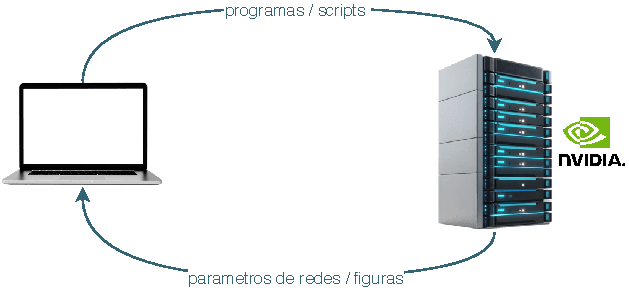
\includegraphics[width=0.6\textwidth]{imaxes/servidor.drawio.pdf}
	\caption{As comunicacións entre o portatil do alumno e o servidor seguen un bucle de sicronización.}
	\label{fig:servidor}
\end{figure}

Fíxose uso do portatil do alumno para o desenvolvemento do código así como dun servidor cedido polo Grupo VARPA que conta cunha gráfica NVIDIA RTX A6000 ó que o alumno podía conectarse de xeito remoto. Ó desenvolver os programas no seu portatil, o alumno debía sincronizarse co servidor para que o segundo tivese o código do primeiro, e o primeiro os artefactos do segundo (ver Figura \ref{fig:servidor}).
\section{Planificación}
\nota{teño que simular unha planificación que non fixemos?}
